\chapter{Methods and Validation}
\section{Numerics of mode evolution}
    \subsection{$tau_s$}
    \subsection{When to set IC's for each mode.}
    \subsection{Swapping variables.}
    \subsection{Freeze-out.}
\section{Integration choices}
    \subsection{The $i\varepsilon$ prescription}
    \subsection{Expand on what F\&RP wrote.}
    \subsection{Suppression from plane wave expansion (intuition).}
\section{Starting the integration with a pinch}
The previous two sections detailed the methods required to calculate
the coefficients $\alpha_n$ in~\eqref{goal}, obtaining an
explicitly separable expression for the shape function.
In this set-up,
there are two kinds of integrals we must compute: integrals over time of
the form~\eqref{inin_kindep}, and integrals over $k$ of the form~\eqref{mode1Dcoeffs_integral}.
The first is done once per coefficient for each vertex, the second is a decomposition
done once for $\zeta_k$ and $\zeta_k'$ each, every timestep.
In this section we detail how to numerically evaluate these
integrals accurately and efficiently.


Since calculating each point in the time integrand requires a
decomposition~\eqref{mode1Dcoeffs_integral}, which is highly oscillatory
at early times, it is worthwhile to consider how to perform the
time integral efficiently. From the form of the Bunch-Davies mode functions,
we expect the dominant frequency (in $\tau_s$) to be $3\kmax$.
Assuming we are earlier than any features that might change this,
we can use this knowledge to sample the integrand at a far lower rate,
building the oscillation into our quadrature weights.
A second important consideration comes from how early we sample the integrand.
We can of course only obtain a point in the time integrand after our mode
functions have burned in from their set initial conditions to their true
attractor trajectory. This means that sampling earlier in the time integrand
requires us to set the initial conditions for the mode functions deeper
in the horizon, a regime in which they are expensive to evolve.


The integrals of the form~\eqref{inin_kindep} that we must calculate have $\tau=-\infty$ as their lower limit.
The highly oscillatory nature of the mode functions in these early times ($\lvert k\tau_s\rvert\gg1$) suppresses the
coefficients of our basis expansion by a factor of $1/\tau_s$.
As noted in~\cite{Funakoshi}, this means that we do not need to
explicitly use the $i\varepsilon$ prescription to force the integrals to converge.
In the case of using the Legendre polynomials as our
basis, we can see this more precisely by considering
the plane wave expansion (e.g.~\cite{finite_ft_legendre}):
\begin{align}\label{exp_expansion}
    e^{-i\bar{k}(\kmax-\kmin)\tau/2} = \sum_{n=0}^{\infty}(2n+1)i^n P_n(\bar{k})j_n(-(\kmax-\kmin)\tau/2)
\end{align}
for $\bar{k}$ in $[-1,1]$. When $(\kmax-\kmin)\tau/2$ is large, the spherical Bessel functions
oscillate with an amplitude $\propto\frac{1}{\tau}$. Thus,
the initial conditions~\eqref{bd_ic} expanded in Legendre polynomials (and similar)
give us suppression of $1/\tau^3$ in~\eqref{inin_kindep}.


While our method has extra suppression compared to configuration-by-configuration methods
(and thus does not need the $i\varepsilon$ prescription to converge)
it still converges rather slowly, as we push the lower limit to earlier times.
This expensive sampling can be wasteful of resources,
especially in a feature scenario where we know this
region will not contribute to the final result.
Care is required however, as starting the integration in the wrong way can easily lead to
errors which can completely swamp the result, since higher order modes
are more sensitive to early times.
The authors of~\cite{chen_easther_lim_1} used an artificial damping term to smoothly
``turn on'' their integrand.
The point at which this is done can then be pushed earlier to check for convergence.
However they found that the details of the damping needed to
be carefully set to avoid underestimating the result.
In~\cite{chen_easther_lim_2} they replaced this method by a ``boundary regulator'';
they split the integral into early and late parts and used integration by parts to
efficiently evaluate the early time contribution.
As our integrand already has extra suppression compared to the configuration-by-configuration
integrands considered in~\cite{chen_easther_lim_1,chen_easther_lim_2},
we can safely use the simpler first method.


We understand this situation by
taking advantage of asymptotic behaviour of highly oscillatory
integrals (for a review see~\cite{iserles_2005}).
Since the leading order term depends on
the value of the non-oscillatory part only at the endpoints,
and the next-to-leading order correction depends on the
derivative only at the endpoints, we can approximate the integral
$\int_{-\infty}^T f(\tau_s)e^{iw\tau_s}d\tau_s$
by replacing the non-oscillatory part $f(\tau_s)$ with a function with
matching value and derivative at $\tau_s=T$,
but which converges far faster.
We use
\begin{align}\label{smooth_cutoff}
f(\tau_s)e^{-\beta^2(\tau_s-T)^2},
\end{align}
for $\tau_s<T$.
In this way, for sufficiently large $T$,
we obtain the accuracy of the
first two terms of the asymptotic expansion
($O(\beta^2/w^2)$, $w=3\kmax$) without needing to explicitly
calculate the derivative at $T$, or needing any phase information (as
one would need to accurately impose a sharp cut on the integrand).


\begin{figure}[!pth]
\centering
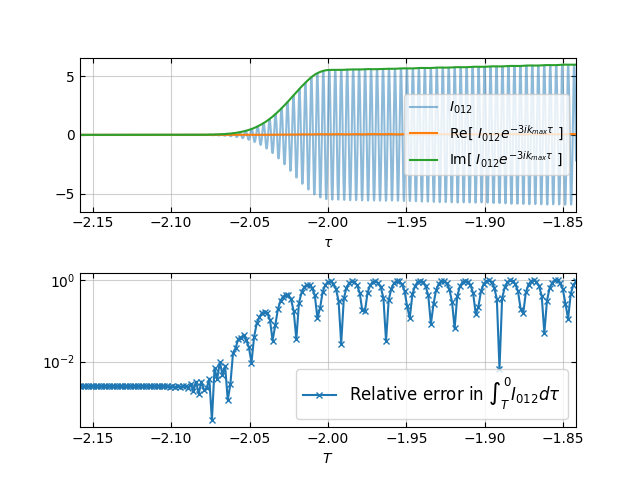
\includegraphics[width=\columnwidth]{plots/time_integrand.png}
\caption{
    A toy example demonstrating the considerations involved in performing the
    time integrals~\eqref{inin_kindep}.
    By carefully starting the time integrations,
    using the form~\eqref{smooth_cutoff}, we can avoid
    errors that would otherwise swamp our result.
    The coefficient being calculated is the
    $\alpha_{012}$ coefficient of the $\Lbasic$ expansion of~\eqref{example_eft2}.
}\label{time_integrands}
\end{figure}


We use a damping of the form $e^{-\beta^2(\tau_s-T)^2}$ for $\tau_s<T$ to smoothly
set the integrand to zero before a certain initial time, $T$.
As long as $T$ is sufficiently early and $\beta$ is not too large
their precise values have no significant effect on the final result.
For definiteness, we take $\beta/w=1\times10^{-4}$, small enough that
the integrand has many oscillations while it is ``turning on'',
so matches the contribution of an infinite limit to high accuracy.
We demonstrate this in figure~\ref{time_integrands}
for a toy $\Hint=(-1/\tau)\dot{\zeta}^3$,
as in~\eqref{example_eft2}.


To obtain a $k$-sample we must evolve a Fourier mode from Bunch-Davies initial conditions deep in the horizon
until it becomes constant after horizon crossing.
We denote by $N_k$ the number of Fourier modes we evolve.
Different choices of distributing the k-samples are possible; for example, one could distribute them
with an even spacing, log-spacing or cluster them more densely near $\kmin$ and $\kmax$.
The $k$-integrals themselves can be computed quite efficiently since
at every timestep the integral is over the same sample points.
One can therefore calculate and store the values of the basis functions at each of these points,
along with the integration weights which will depend on the distribution of $k$-samples.
The actual integration at each timestep, the calculation of the 
coefficients in~\eqref{mode1Dcoeffs_integral}, then becomes nothing more
than a dot product of a time-independent array with the
numerically evolved mode functions, for each order up to $\Pmax$.
We have found the best convergence results from distributing the k-samples
according to the prescription of Gauss-Legendre quadrature.


To calculate the basis expansion of the bispectrum using the in-in formalism
we must first calculate the basis expansion of the mode
functions at each timestep~\eqref{mode1Dcoeffs_integral}.
At early times the mode functions are highly oscillatory, taking the form $z_k e^{-ik\tau_s}$
for some much smoother $z_k$.
Directly decomposing this would require evolving more $\zeta_k$ samples
than is practical.
We want an expansion of the form
\begin{align}\label{mode_expansion}
	z_k e^{-ik\tau_s} = \sum_{n=0}^{\infty}\alpha_n q_n(k).
\end{align}
We can obtain this by using standard oscillatory
quadrature, if the $\tau_s$ dependence of the weights does not add too much overhead.
We can also use an expansion of $e^{-ik\tau_s}$
with a known explicit time dependence, for example
the expansion~\eqref{exp_expansion}.


To use this second method,
the first (smooth) factor $z_k$ can be expanded in whatever basis we are working in, $q_n(k)$,
and the second factor (highly oscillatory in $k$) is expanded
in some convenient basis $\tilde{q}_n(k)$
(e.g.\ $\Fbasic$, or $\Lbasic$ using the analytic form~\eqref{exp_expansion}).
Then by precomputing
$q_a(k)\tilde{q}_b(k)$
as a linear combination of the set of basis functions $q_c(k)$
all we need calculate at each timestep is the coefficients
of the smoother $z_k(\tau_s)$, which we then convert to the coefficients
of $F^{(i)}(\tau, k)$. In this way we can retain flexibility in our
bispectrum basis, as well as efficiency and precision in the calculation.
In the case of using $\Lbasic$ for the $\tilde{q}_n(k)$,
assuming the expansion in~\eqref{shapemodeexp} converges,
we need only compute the expansion for $e^{-ik\tau_s}$ to enough
terms that the first $\Pmax$ of the
coefficients in the expansion~\eqref{mode1Dcoeffs_sum} of the $F^{(i)}(\tau, k)$ converge,
not until the actual sum~\eqref{mode1Dcoeffs_sum} converges, since for high enough orders the integrals
in~\eqref{inin_kindep} will integrate to zero.


Clearly, once $\tau_s$ becomes small enough these considerations will no longer be necessary
and we can simply decompose the mode function directly.
We do this around the horizon crossing of the geometric mean of $\kmin$ and $\kmax$.
If there is an extreme feature which causes a large deviation from the usual slow-roll form
this switch will need to be made sooner. 
Also, this method would need to be adapted for non-Bunch-Davies initial conditions.
Since anything related to the basis but independent of the scenario can be
precomputed, certain parts of this calculation do not hurt the efficiency of this
method in the context of, for example, a parameter scan.
Using the methods outlined above,~\eqref{inin_kindep} and~\eqref{mode1Dcoeffs_integral}
can be computed precisely and efficiently in a mostly basis-agnostic context
allowing us to ({\romannumeral 1}) preserve the intrinsic separability of the tree-level
in-in formalism and ({\romannumeral 2}) do so in a way that allows easy exploration of possible
sets of basis functions, to find a set that converges quickly enough to
be useful in comparison with observation.
    \subsection{When to start.}
    \subsection{Show how easy it is to swamp the result with a sharp start.}
    \subsection{FIGURE: Relative error for simple $\pi^3$ and for Reso, in ($\beta$, T).}
\section{Oscillatory weights}
    \subsection{When to swap.}
    \subsection{Validation.}
\section{Stopping the integration}
    \subsection{A note on boundary terms and difficult (time-dep) cancellations.}
\section{The interaction Hamiltonian}
The methods detailed in the previous section depend on the separability of
the third-order interaction Hamiltonian, $\Hint$,
and the possibility of including the spatial derivatives in a
numerically accurate and efficient way.
To make precise how our methods take into account the details of
$\Hint$, we will take $P(X,\phi)$ inflation as an example.
The full cubic interaction Hamiltonian, not neglecting boundary terms,
can be calculated as~\cite{px_burrage,chen_ng_0605,seery_ng_0503}
\begin{align}
    \Hint(t)=\ \int d^3x\bigg\{& -\frac{a^3\varepsilon}{H c_s^4}\left(1-c_s^{2}-2c_s^{2}\frac{\lambda}{\Sigma}\right)\dot{\zeta}^3
		+ \frac{a^3\varepsilon}{c_s^{4}}\left(3-3c_s^2-\varepsilon+\eta\right) \zeta\dot{\zeta}^2\nonumber\\
		&- \frac{a\varepsilon}{c_s^{2}}\left(1-c_s^2+\varepsilon+\eta-2\varepsilon_s\right) \zeta(\partial\zeta)^2\nonumber\\
        &- \frac{a^3\varepsilon^2}{2c_s^{4}}(\varepsilon-4)\dot{\zeta}\partial\zeta\partial(\partial^{-2}\dot{\zeta})
        - \frac{a^3\varepsilon^3}{4c_s^4}\partial^2\zeta(\partial(\partial^{-2}\dot{\zeta}))^2\bigg\}\label{interaction_loc}
\end{align}
with $\Sigma=\frac{H^2\varepsilon}{c^2_s}$
and $\lambda = X^2P,_{XX}+\frac{2}{3}X^3P,_{XXX}$.
See~\cite{px_burrage} for further details.


This is commonly quoted with a term proportional to the equation of motion,
but this will never contribute~\cite{px_burrage,bdy_arroja,bdy_passaglia,bdy_rigopoulos}.
We do not need to make a slow-roll approximation
(the quantities defined in~\eqref{slowrollparams} are not required to be small,
except in that we wish to have a successful inflation scenario),
nor do we need to neglect any terms in the interaction Hamiltonian.
We do no field redefinition,
so do not need to add a correction to the final bispectrum.
Following the calculation of~\cite{px_burrage} (see also~\cite{bdy_arroja,bdy_passaglia,bdy_rigopoulos})
we do not work with any boundary terms.
Numerically this is preferable to forms with boundary terms,
whether they come from undoing a field redefinition or from integration by parts.
Since the boundary term contribution will depend on the choice of when to end the integration,
its time dependence must cancel with a late-time time-dependent
contribution of some vertex, requiring us to track the necessary quantities
much longer than otherwise needed to obtain the desired precision.

Schematically, the correction from a field redefinition would look like
\begin{align}
{
\left< \zeta_{\bf{k_1}}\zeta_{\bf{k_2}}\zeta_{\bf{k_3}} \right>
    = \left< \tilde{\zeta}_{\bf{k_1}}\tilde{\zeta}_{\bf{k_2}}\tilde{\zeta}_{\bf{k_3}} \right>
    + \lambda \left< \tilde{\zeta}_{\bf{k_1}}\tilde{\zeta}_{\bf{k_2}} \right>\left< \tilde{\zeta}_{\bf{k_1}}\tilde{\zeta}_{\bf{k_3}} \right>
    + cyclic
}
\end{align}
where $\lambda$ is some function of the slow-roll parameters.
The correction terms will have a time dependence from $\lambda$,
so the $\left< \tilde{\zeta}_{\bf{k_1}}\tilde{\zeta}_{\bf{k_2}}\tilde{\zeta}_{\bf{k_3}} \right>$
term must have some late time contribution to cancel it.
To obtain an accurate result, care would need to be taken with this cancellation,
an unnecessary complication.

By integrating by parts and using the equation of motion,
the interaction Hamiltonian can be rewritten without
picking up boundary terms~\cite{rp_integ_by_parts}.
Using $(3.7)$ from~\cite{rp_integ_by_parts},
with $f=-\varepsilon/(c_s^2H)$,
we obtain the following form:
\begin{align}
    \Hint(t)=\ \int d^3x\bigg\{& -\frac{a^3\varepsilon}{H c_s^4}\left(-c_s^{2}-2c_s^{2}\frac{\lambda}{\Sigma}\right)\dot{\zeta}^3
		+ \frac{a^3\varepsilon}{c_s^{4}}\left(-3c_s^2\right) \zeta\dot{\zeta}^2\nonumber\\
		&- \frac{a\varepsilon}{c_s^{2}}\left(-c_s^2\right) \zeta(\partial\zeta)^2
        - \frac{a\varepsilon}{Hc_s^2}\dot{\zeta}(\partial\zeta)^2\nonumber\\
        &- \frac{a^3\varepsilon^2}{2c_s^{4}}(\varepsilon-4)\dot{\zeta}\partial\zeta\partial(\partial^{-2}\dot{\zeta})
        - \frac{a^3\varepsilon^3}{4c_s^4}\partial^2\zeta(\partial(\partial^{-2}\dot{\zeta}))^2\bigg\}.\label{interaction_eql}
\end{align}
To leading order, this formulation is made up of terms that
give equilateral shapes when the slow-roll parameters are roughly constant.
It was pointed out in~\cite{Funakoshi} that
using~\eqref{interaction_loc} in a scenario that results in an equilateral shape
would require sensitive cancellations in the squeezed limit.
Likewise, using~\eqref{interaction_eql} for a local scenario
would require sensitive cancellations in the equilateral limit.

As mentioned in~\cite{Funakoshi}, the spatial derivatives
can be manipulated into simple prefactors of $k_i$ using the
triangle condition ($\mathbf{k_1}+\mathbf{k_2}+\mathbf{k_3}=0$),
and so preserve the separability of the result.
To absorb these prefactors in our calculation, we precompute
$k^{p}q_a(k)$ as a linear combination of the $q_a(k)$ for the
relevant values of $p$,
from which $V^{(i)}_{P\tilde{P}}$ defined in~\eqref{V_definition} is built.
For certain sets of basis functions this matrix can be calculated analytically,
but it is simpler and more robust to numerically calculate the relevant integral directly.
The processing cost this incurs is small, and must only be
paid once per basis. We note especially that this means the matrix can
be stored and efficiently used in many scenarios.
To summarise,
we calculate the bispectrum contribution from each vertex in $\Hint$ separately:
we assemble the integrands, integrate them with respect to time,
include the prefactors coming from the spatial derivatives,
then sum the resulting sets of basis coefficients.
Of course, these methods are not restricted to this example of $\Hint$.
    \subsection{Using integration by parts from RP paper.}
\section{Set-up of DBI example scan}
    \subsection{Matching $A_s$, $n_s$, $r$, $N*$, using $\beta_{IR}$ etc.}
\section{Going to high $P_{max}$}
    \subsection{How high can I go, in terms of Planck $w$?}
    \subsection{How high can I go, in terms parameters that can't be compared to Planck?}

\section{Validation (on numerical results)}
\subsection{Validation methods}\label{sec:validation_methods}
In this section we validate our implementation of our methods
on different types of non-Gaussianity, sourced in different ways.
While our actual results take the form of a set of mode expansion coefficients $\alpha_n$,
to make contact with previous results in the literature
all of our validation tests take place on the tetrapyd,
the set of physical bispectrum configurations.

We test that our results have converged using~\eqref{relative_difference},
between $\Pmax=45$ and $\Pmax=15$ for the featureless cases,
and between $\Pmax=65$ and $\Pmax=35$ for the cases with features.
We will refer to this as our convergence test.
To verify that our results have converged to the correct shape,
we perform full tetrapyd checks against known analytic results
(where those are available, and in their regimes of validity)
using~\eqref{relative_difference},
and point tests against the PyTransport code for the scenarios
with canonical kinetic terms.
Since all our scenarios are single-field, the most general
test we have is the single-field consistency relation,
which states that for small $k_L/k_S$, the shape function $S(k_S,k_S,k_L)$
must obey~\eqref{eq:sqz_consistency}.
The consistency condition should hold most precisely
at the configurations with smallest $k_L/k_S$,
the most squeezed being the three corners, $(\kmax,\kmax,\kmin)$ and permutations.
We want our test to be on an extended region of the tetrapyd however,
so we choose the line
\begin{align}\label{sqz_line}
    \frac{k_L}{k_S}&=\frac{2\kmin}{\kmax},
\end{align}
which connects $(\kmax,\kmax,2\kmin)$ to $(\kmax/2,\kmax/2,\kmin)$.
We will take $\frac{\kmin}{\kmax}=\frac{1}{550}$, so this is still sufficiently squeezed to be a stringent test.

First, we investigate convergence on simple featureless models,
both local-type~\eqref{eq:quadratic_potential}
and equilateral-type~\eqref{eq:dbi_warp}.
We find that in our chosen basis $\Lnsboth$ our results
converge quickly and robustly as we increase the number of modes,
where we quantify the convergence using~\eqref{relative_difference}.
We compare the converged results against analytic
templates~\eqref{malda_shape} and~\eqref{dbi_shape},
using the full shape information~\eqref{relative_difference},
finding them to match to high accuracy.
Secondly we validate our methods on an example of non-Gaussianity
from a feature: linear oscillations from a sharp step in the
potential~\eqref{eq:kink_potential}. The result converges robustly
across the parameter range we explore. Throughout that range,
we test the converged result using the squeezed limit consistency
condition, and perform point tests against PyTransport,
finding excellent agreement.
For small step size we can further validate against the analytic template
of~\cite{adshead}, using the full shape information, finding agreement
to the expected level given the finite width of the step.
The final type of non-Gaussianity we use for validation on is the resonance
type, logarithmic oscillations generated deep in the horizon~\eqref{eq:resonant_potential}.
We test the converged result against the PyTransport
code, by performing point tests on a slice.
We also present a resonant DBI scenario, with out-of-phase oscillations
in the flattened limit, as pointed out in~\cite{chen_folded_resonant},
resulting from non-Bunch-Davies behaviour of the mode functions.
We also test both resonant scenarios using the squeezed limit consistency condition.


\begin{figure}[!pth]
\centering
    \subfloat{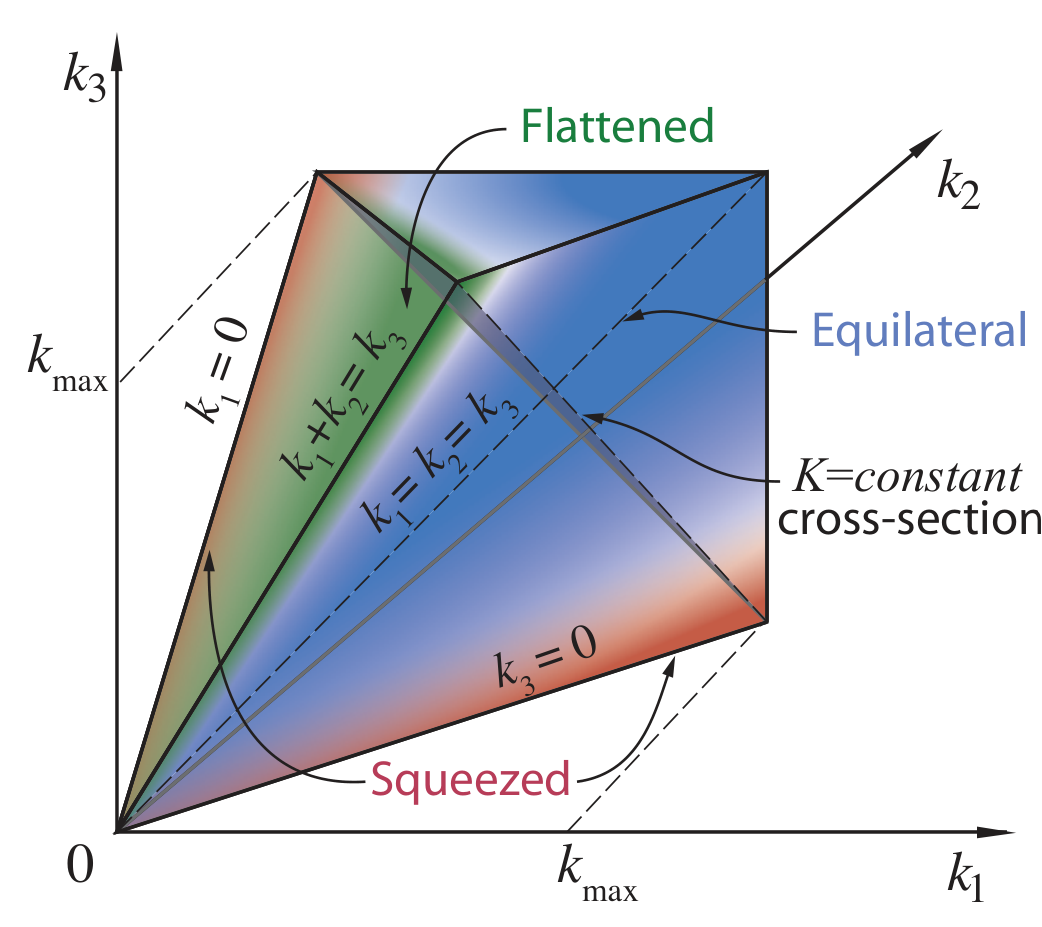
\includegraphics[width=.45\columnwidth]{plots/tetrapyd_3d_colour_split.png}}
    \subfloat{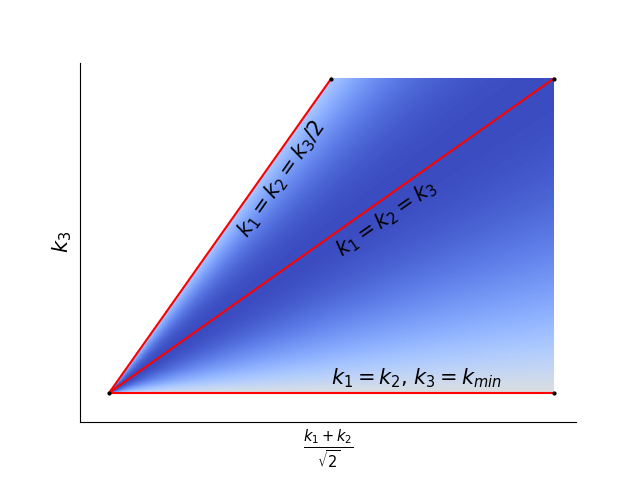
\includegraphics[width=.55\columnwidth]{plots/slice_explained.png}}
\caption{
    For ease of display, we will plot the two-dimensional $k_1=k_2$ slice of the tetrapyd
    for each of our validation examples, as shown schematically here on the right.
    Horizontal lines on this plot have
    constant $k_3$. The bottom edge is $k_3=\kmin$, the top
    edge is $k_3=\kmax$. The right edge is $k_1=k_2=\kmax$, the
    left edge is $k_1=k_2=k_3/2$, i.e.\ the limit imposed by the triangle condition.
    Plotted in red (in the right hand plot) from top-left to bottom-right,
    are the flattened, equilateral and squeezed limits. For comparison,
    half of the tetrapyd is shown in the three-dimensional plot on the left.
}\label{slice_explained}
\end{figure}


We display the phenomenology of our various validation examples
by plotting slices through the tetrapyd, as detailed in figure~\ref{slice_explained}.
Along with the phenomenology plots we plot the residual
(with respect to the totally converged result)
on the same slice, relative to the magnitude of the shape~\eqref{rep_val}.
We emphasise that while these plots display slices through the
tetrapyd, our actual result describes the shape function on the
entire three-dimensional volume of the tetrapyd, and
we measure our convergence over this whole space.

While one of the main advantages of this method is its direct link
to the CMB, in this section we only concern ourselves with validating the
code, not the observational viability of the scenarios considered.
We focus on accurately and efficiently calculating the primordial
tree-level comoving bispectrum, validating on models popular in the
literature.
\subsection{Quadratic slow-roll}
The first model we will consider is slow-roll inflation
on a quadratic potential~\eqref{eq:quadratic_potential}.
We consider two scenarios, both with $m=6\times10^{-6}$.
The first is deep in slow-roll, which we achieve by choosing
$\phi_0=1000$; then, choosing $\phi'_0$ according to the
slow-roll approximation, we get
$\frac{1}{2}\phi'^2=\varepsilon\approx0.2\times10^{-5}$.
We can then choose the initial value for $H$ to
satisfy the Friedmann equation to sufficient precision.
The second scenario is chosen to have a value for $n_s^{*}-1$
consistent with the $\textit{Planck}$ result,
by choosing $\phi_0=16.5$, so that $\varepsilon\approx0.8\times10^{-2}$.
The shapes are shown in figure~\ref{slice_plot_malda}.


We choose the first scenario to have such a small value of $\varepsilon$
so that we can use Maldacena's shape~\eqref{malda_shape}
as a precision test.
Indeed, we find that it has a scaled relative difference~\eqref{relative_difference_scaled}
of $2.7\times10^{-5}$ with this shape,
contrasting a scaled relative difference
of $0.077$ with the local template~\eqref{local_shape}.
This confirms that our methods and our implementation in code can accurately
pick up this basic type of featureless non-Gaussianity.


For the second scenario, we cannot validate on
Maldacena's shape~\eqref{malda_shape} or the
local template~\eqref{local_shape},
as for $\epsilon\approx0.8\times10^{-2}$ we only expect
these templates to match the true result to percent level accuracy.
Indeed, we find that our result has a correlation of $0.998$
with both~\eqref{malda_shape} and~\eqref{local_shape},
corresponding (in the sense of~\eqref{relative_difference_scaled})
to a relative difference of $6\%$,
as expected.
Instead, we validate this model using
the squeezed limit test described above,
verifying our result to $0.05\%$.


This is a validation of the convergence of our basis,
reaffirming the template decomposition results of figure~\ref{fig:recon_malda_dbi}
in the setting of the in-in formalism.
It is also a stringent validation of our methods of including the higher-order
coefficients, as insufficient care taken in the early-time sections of
integrals~\eqref{inin_kindep}, or in including the spatial derivatives
from $\Hint$, could have easily swamped the $\Pmax=45$ result.


\begin{figure}[!pth]
\centering
    \subfloat{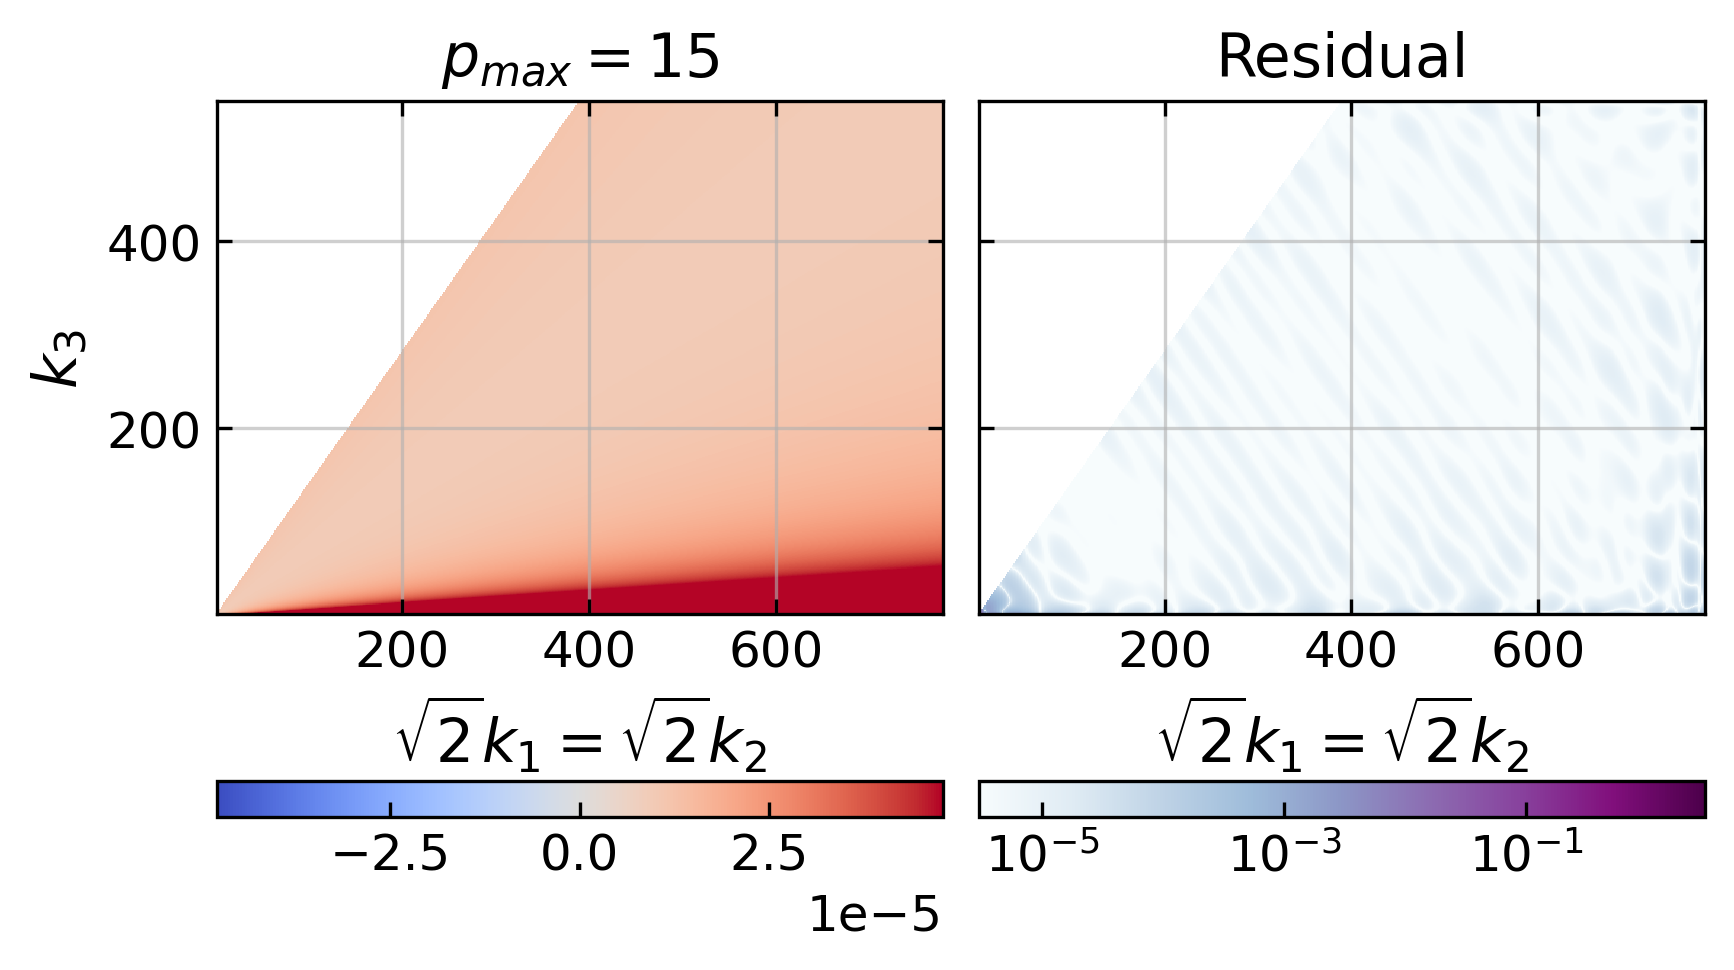
\includegraphics[width=0.99\columnwidth]{plots/tetra_slice_malda_sr_hq.png}}\\[-2ex]
    \subfloat{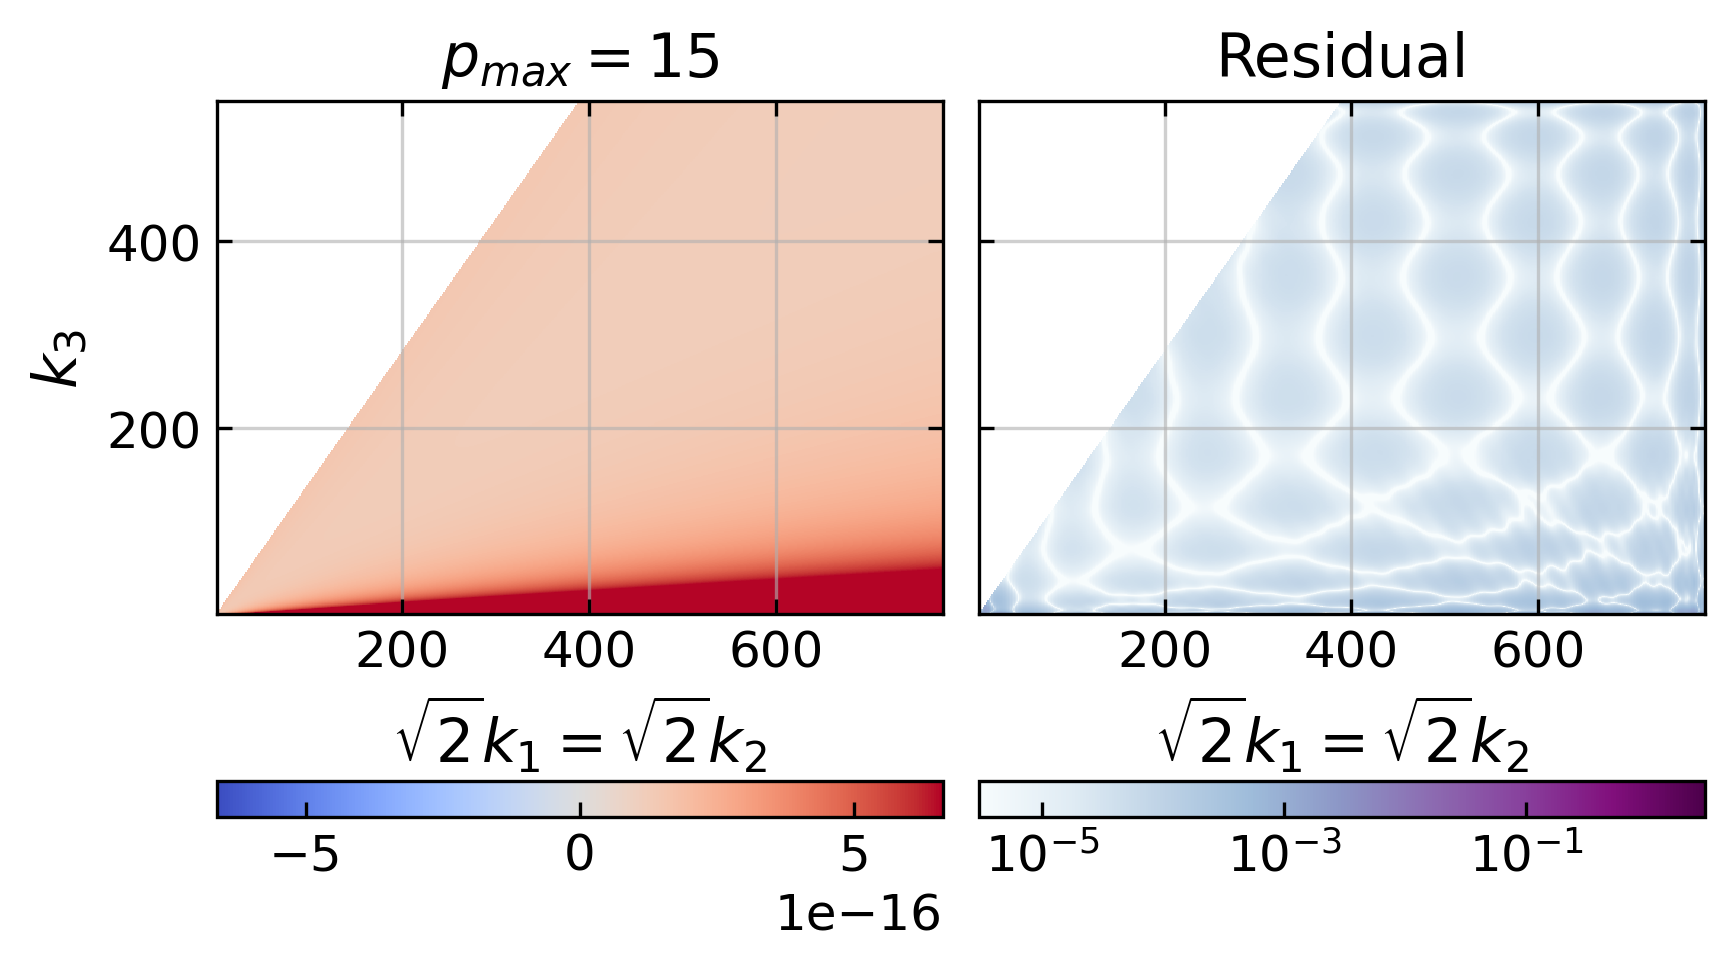
\includegraphics[width=0.99\columnwidth]{plots/tetra_slice_malda_hq.png}}
\caption{
    A canonical single-field model on a quadratic
    potential~\eqref{eq:kink_potential},
    slowly-rolling with $\varepsilon\approx2\times10^{-6}$
    in the top plot, and $\varepsilon\approx0.8\times10^{-2}$
    in the lower plot.
    This shape is dominated by its squeezed limit,
    and has a scale dependence determined by $\varepsilon$,
    very small in the top plot and ``realistic'' in the
    lower plot, relative to the $\textit{Planck}$ power spectrum.
    The first scenario converges well in the $\Linvk$ basis,
    with a relative difference of $2.7\times10^{-5}$
    %2.6764e-05
    between $\Pmax=45$ and $\Pmax=15$.
    The second scenario converges well in the $\Lnsboth$ basis
    (with $n_s^{*}-1 = -0.0325$),
    with a relative difference of $7.9\times10^{-5}$
    % 7.9047e-05
    between $\Pmax=45$ and $\Pmax=15$.
}\label{slice_plot_malda}
\end{figure}


\subsection{DBI inflation}
Next, we show results for a similar pair of scenarios for DBI inflation.
We choose $V_{0}={5.2\times10^{-12}}$~% and $\beta_{IR}=0.29$
with $m=\sqrt{0.29V_0/3}$
in~\eqref{eq:dbi_action} and~\eqref{eq:dbi_warp}.
We choose $\phi_0=0.41$, and then the starting condition
for $H$ according to the slow-roll approximation,
allowing us to choose $\phi'_0$ such that the Friedmann
equation is satisfied to sufficient precision.
The first scenario is deep in slow-roll, with $\lambda_{DBI}=1.9\times10^{18}$, while
the second scenario saturates the $\textit{Planck}$
limit on $c_s$, with $\lambda_{DBI}=1.9\times10^{15}$.
The resulting shapes are shown in figure~\ref{slice_plot_dbi}.


The scenario deep in slow-roll has a error of $0.082\%$
%0.0008243088
relative to the DBI shape~\eqref{dbi_shape},
and $13\%$
%0.1313763404
relative to the equilateral template~\eqref{equil_shape}.
The second scenario has a relative error of $2.9\%$
%0.0293218555
with the scale-invariant DBI shape, and $14\%$ with the equilateral template.
%0.1391026565
Including some scale dependence in the template,
using~\eqref{dbi_ns_shape}, we get a relative error of $0.27\%$.
%0.0026744179
On the line defined by~\eqref{sqz_line},
both scenarios have a sub-percent difference from the
consistency condition, with respect to the equilateral configurations,
which decreases when configurations with a larger $k_S/k_L$ are considered.

Including the minimal information of an individual, approximately
representative value of $n_s^{*}-1$
in $\Lnsboth$ allows us to converge to these smooth shapes quickly
and robustly, overcoming the tetrapyd-vs-cube difficulties described
in~\ref{sec:choice_of_basis}. Our accurate match to these shapes validates our
implementation in code, and the ability of the method
(and our basis in particular) to capture very different types of
bispectrum shapes, local and equilateral.


\begin{figure}[!pth]
\centering
    \subfloat{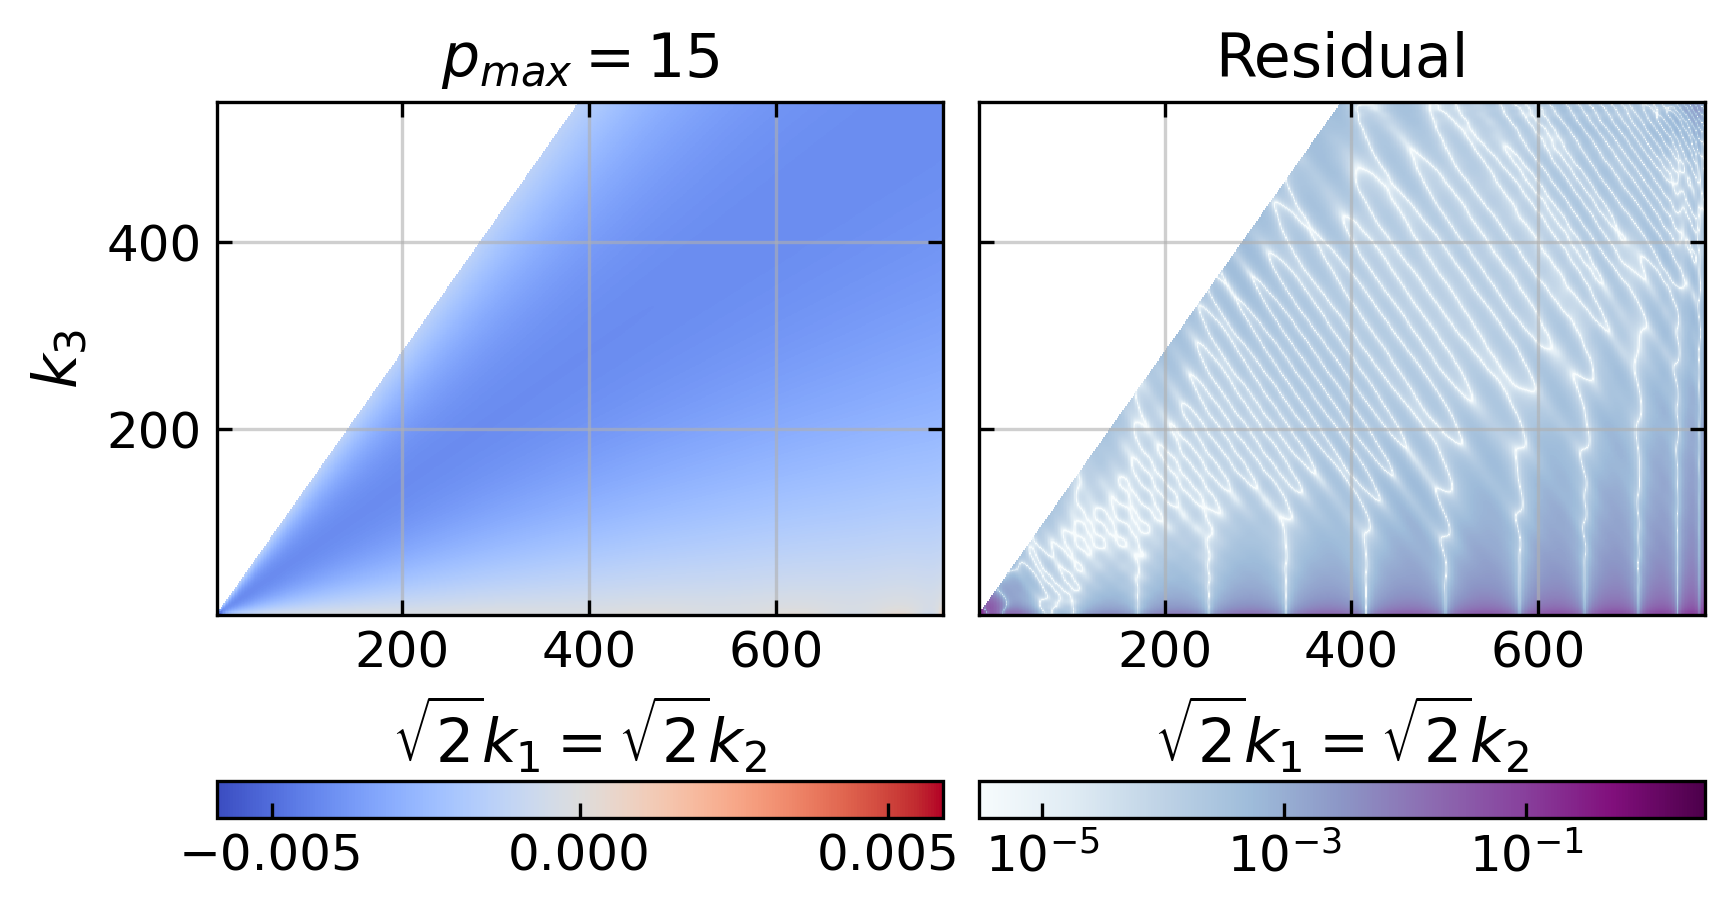
\includegraphics[width=0.99\columnwidth]{plots/tetra_slice_dbi_sr_hq.png}}\\[-2ex]
    \subfloat{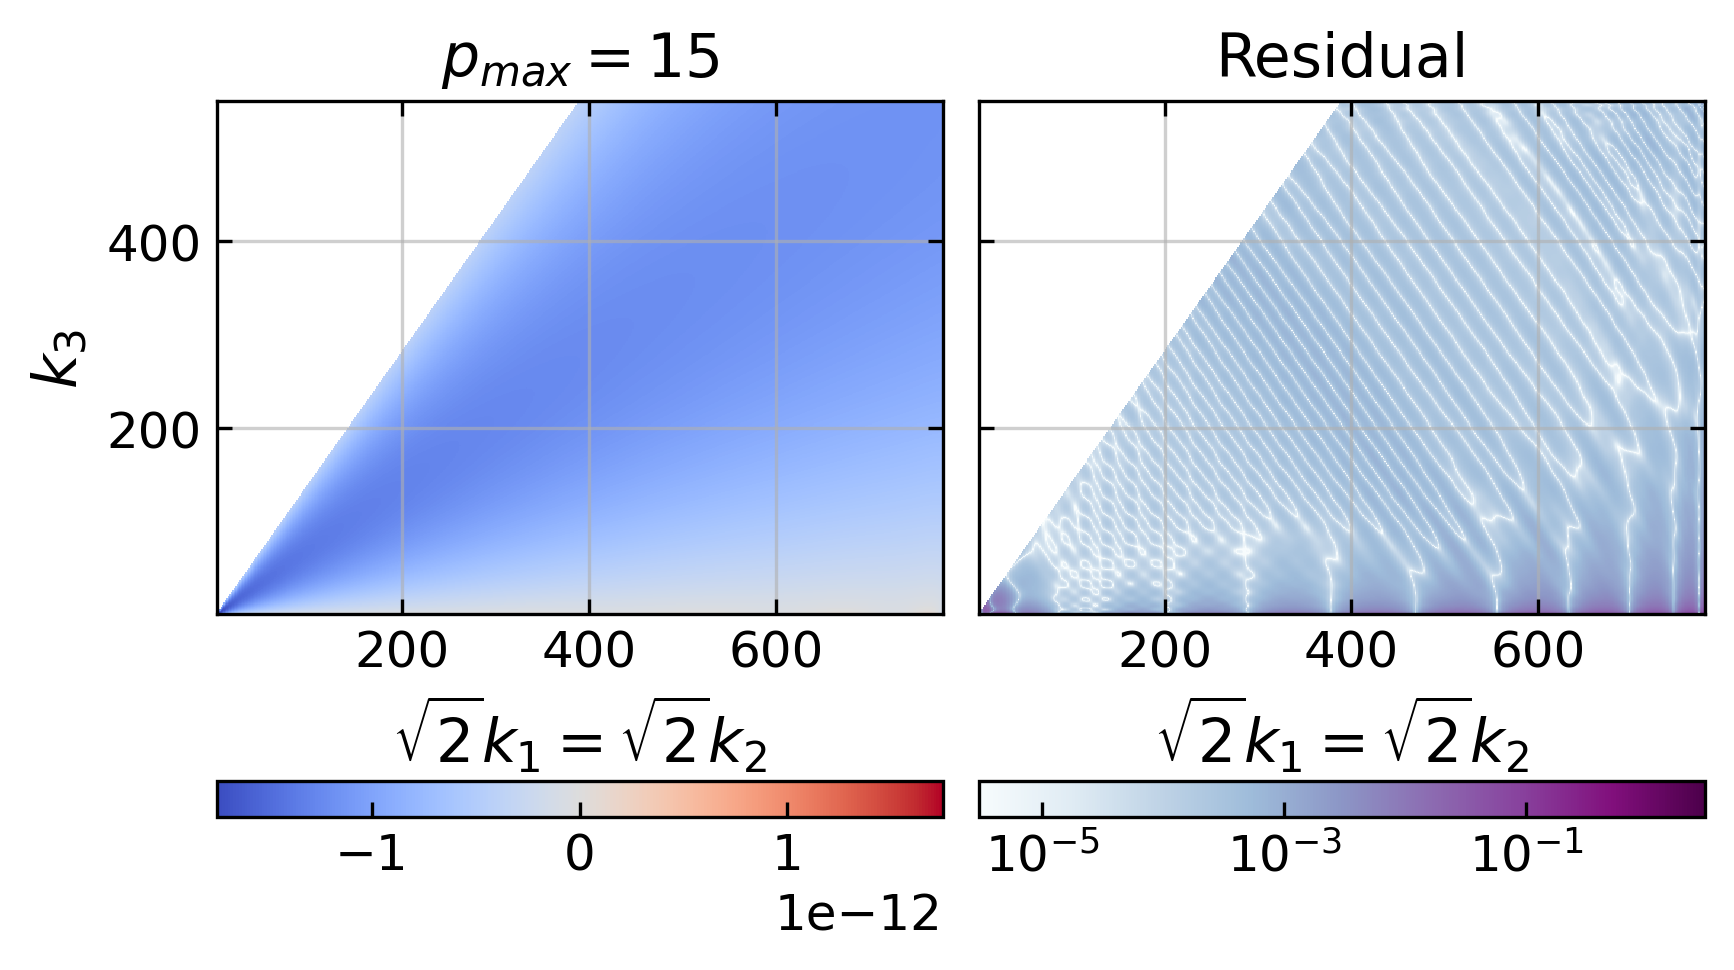
\includegraphics[width=0.99\columnwidth]{plots/tetra_slice_dbi_hq.png}}
\caption{
    The upper plot shows the shape function for a DBI model
    deep in slow-roll. We set
    $\lambda_{DBI}$ in~\eqref{eq:dbi_warp} to $1.9\times10^{18}$,
    obtaining a scenario with $\varepsilon\approx1.9\times10^{-6}$ and
    $c_s=2.3\times10^{-3}$.
    This shape is dominated by its equilateral configurations,
    and has only a slight scale dependence.
    It converges well in the $\Linvk$ basis,
    with a relative difference of $2.1\times10^{-3}$
    % 2.1203e-03
    between $\Pmax=45$ and $\Pmax=15$.
    The lower plot shows a DBI model that saturates the {\it{Planck}}
    limit on $c_s$. We set
    $\lambda_{DBI}$ in~\eqref{eq:dbi_warp} to $1.9\times10^{15}$,
    obtaining a scenario with $\varepsilon\approx8.0\times10^{-5}$ and
    $c_s=8.0\times10^{-2}$.
    This shape is also dominated by its equilateral configurations,
    but has a scale dependence consistent with the measured
    power spectrum.
    It converges well in the $\Lnsboth$ basis
    (with $n_s^{*}-1 = -0.0325$),
    with a relative difference of $1.1\times10^{-3}$
    % 1.1461e-03
    between $\Pmax=45$ and $\Pmax=15$.
}\label{slice_plot_dbi}
\end{figure}


\subsection{Step features}
Moving on from simple featureless bispectra, we present the results of
our validation tests on non-Gaussianity coming from a sharp feature in the potential.
We use the same parameters for the quadratic potential as in the
second scenario in fig~\ref{slice_plot_malda}.
In~\eqref{eq:kink_potential}
we fix $d=1\times10^{-2}$ and $\phi_{f}=15.55$
(as with the second canonical quadratic example, $\phi_0=16.5$).
Figure~\ref{slice_plot_tanh}
shows results for the shape function for two step sizes,
$c=5\times10^{-5}$ and $c=5\times10^{-3}$.
The resulting shape for small step sizes contains simple oscillations,
linear in $k_1+k_2+k_3$,
whose phase is almost constant across the tetrapyd.
When the step size is small, as expected,
our result matches the analytic result of~\cite{adshead},
presented there in equations (48), (54), (55).
We plot a comparison of the result of~\cite{adshead} and our result
in figure~\ref{fig:tanh_scan}.
For larger step size, we check the squeezed limit in figure~\ref{fig:tanh_sqz},
where we also show point tests against the PyTransport code.
Across this range of step sizes, for the resulting shapes we obtain
a full tetrapyd convergence test result
(between $\Pmax=65$ and $\Pmax=35$)
of between $0.17\%$ and $0.15\%$ and
we verify the squeezed limit test to better than $0.5\%$.

These examples show the utility of our methods in
calculating bispectra with non-trivial shape and scale dependence,
going beyond the simple examples of~\cite{Funakoshi}.
They validate the calculation of the high order coefficients,
and show that our code as implemented can handle sharp deviations from slow-roll,
generating non-Gaussianity around horizon crossing.


\begin{figure}[!pth]
\centering
    \subfloat{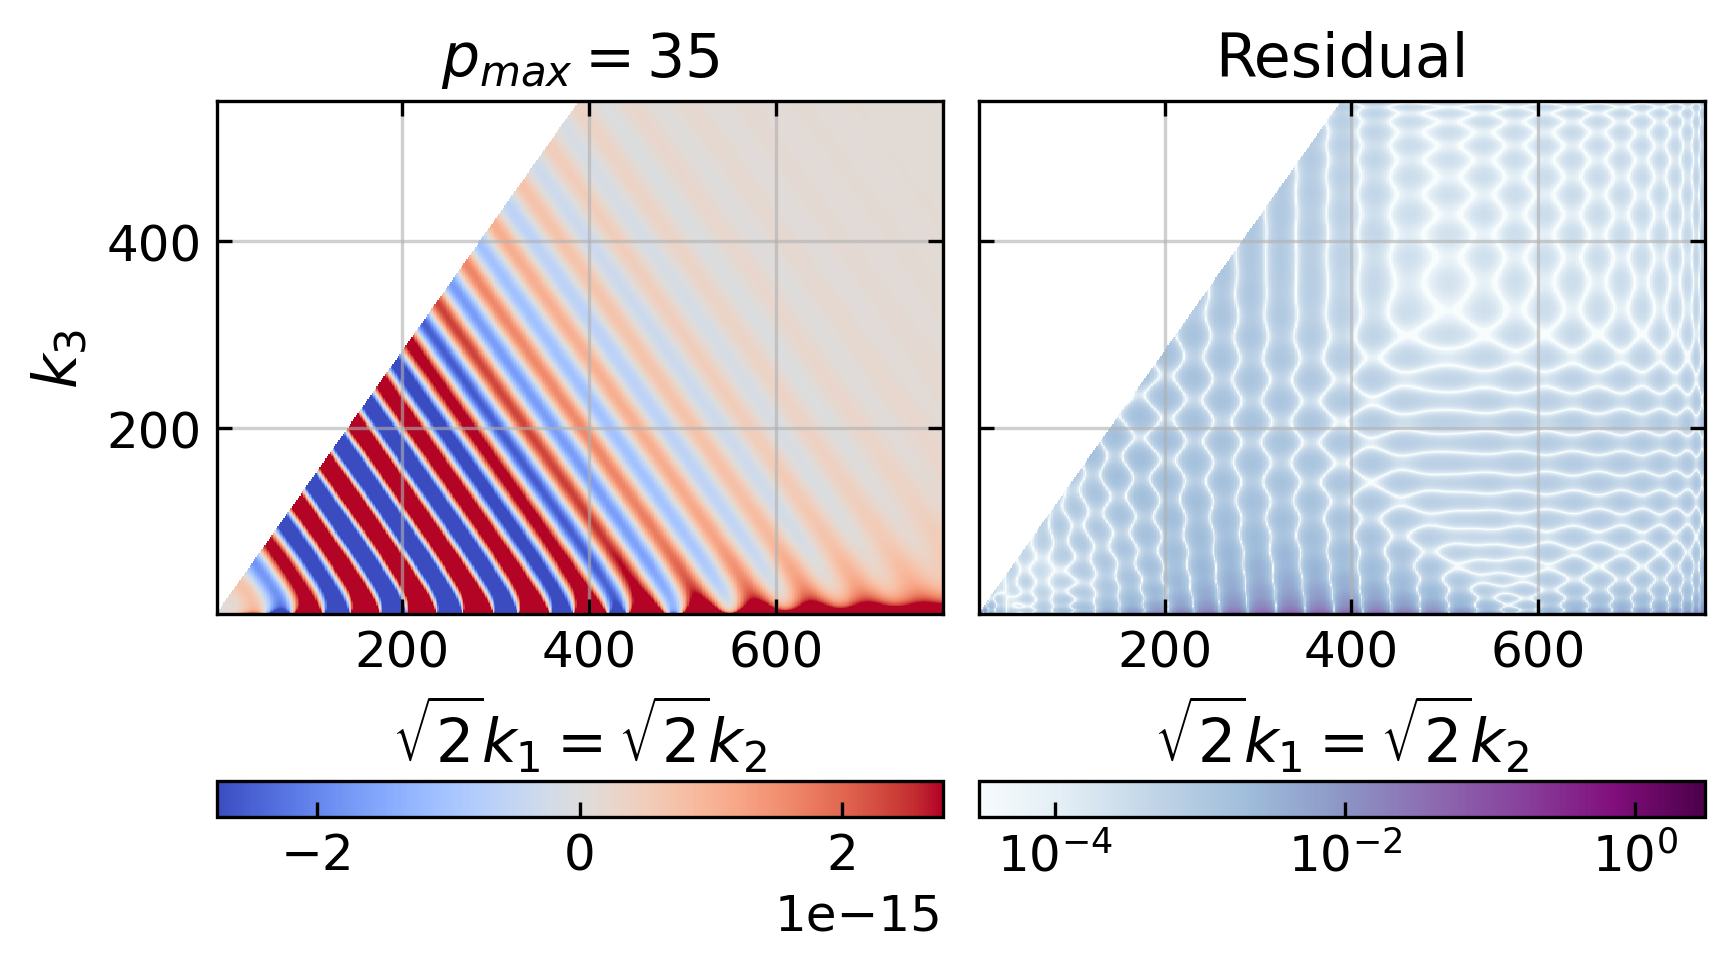
\includegraphics[width=0.99\columnwidth]{plots/tetra_slice_tanh_small_hq.png}}\\[-2ex]
    \subfloat{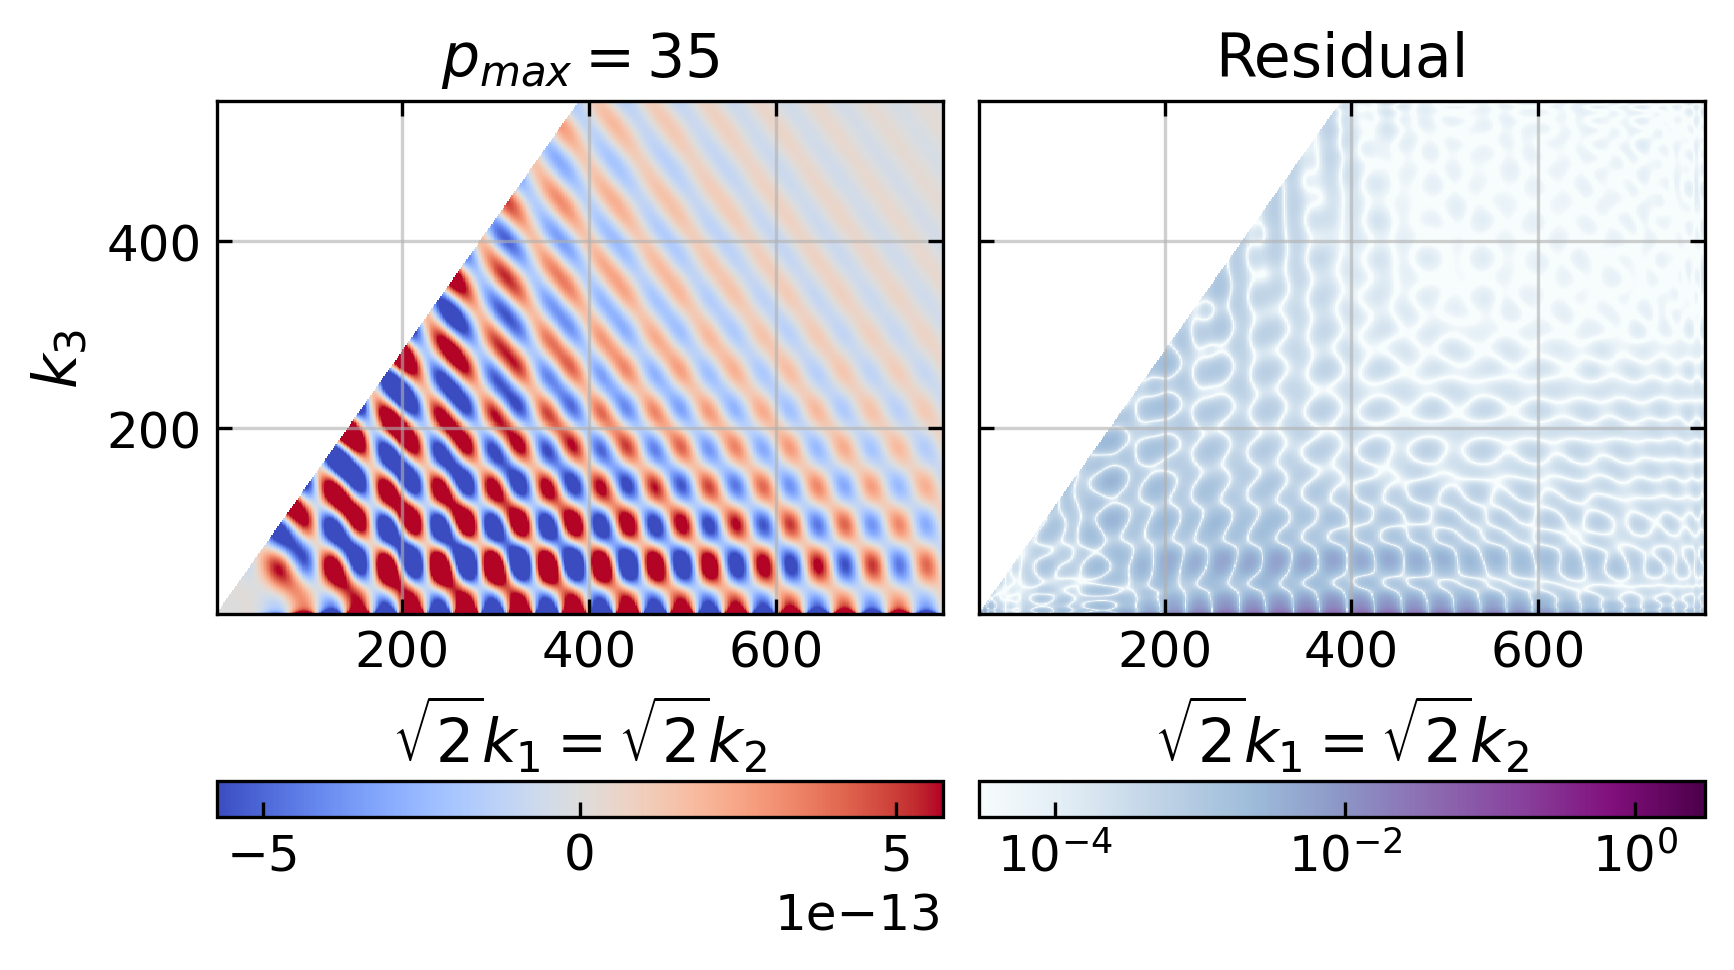
\includegraphics[width=0.99\columnwidth]{plots/tetra_slice_tanh_large_hq.png}}
\caption{
    The tree-level shape function of a feature
    model~\eqref{eq:kink_potential}, shown for step sizes of
    $c=5\times10^{-5}$ (upper plot)
    and $c=5\times10^{-3}$ (lower plot).
    The corresponding expansion parameter values of~\cite{adshead},
    ${\mathcal{C}=6c/(\varepsilon+3c)}$, are $0.035$
    and $1.3$.
    For the smaller step size, the oscillations are almost entirely functions of $K=k_1+k_2+k_3$,
    except for a phase difference in the squeezed limit.
    The dependence is more complicated for $\mathcal{C}=1.3$,
    however our result still converges well.
    In the $\Lnsboth$ basis, with $n_s^{*}-1 = -0.0325$,
    the results have a relative difference of $1.6\times10^{-3}$
    and $1.5\times10^{-3}$, respectively,
    % 1.6406e-03
    % 1.6418e-03
    % 1.4856e-03
    between $\Pmax=65$ and $\Pmax=35$.
}\label{slice_plot_tanh}
\end{figure}
\begin{figure*}
    %\centering
    \subfloat{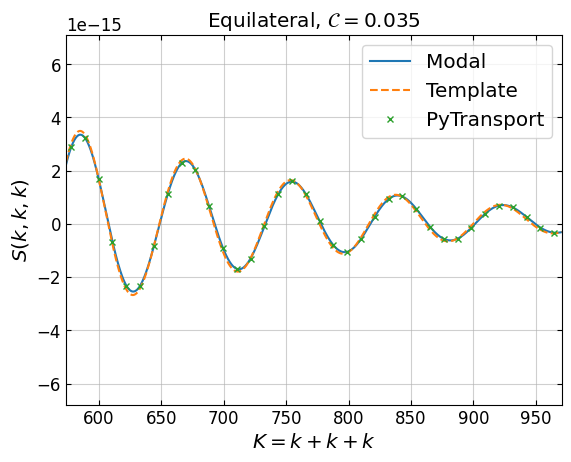
\includegraphics[width=0.49\columnwidth]{plots/tanh_5e-05_equil}}
    \hfill
    \subfloat{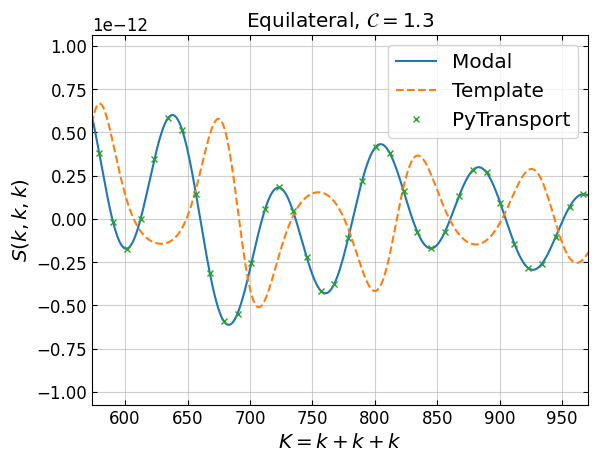
\includegraphics[width=0.50\columnwidth]{plots/tanh_5e-03_equil}}
    \vskip\baselineskip
    \subfloat{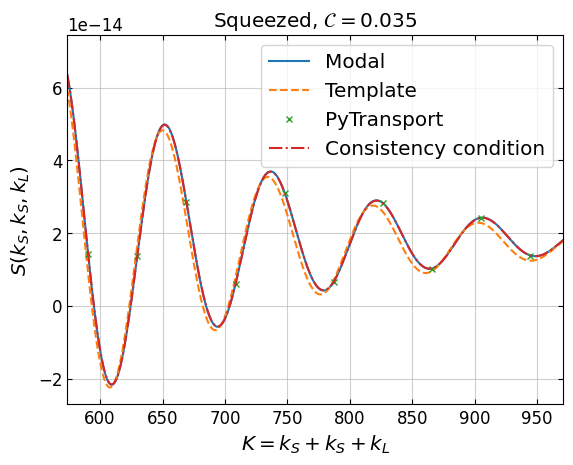
\includegraphics[width=0.49\columnwidth]{plots/tanh_5e-05_sqz}}
    \hfill
    \subfloat{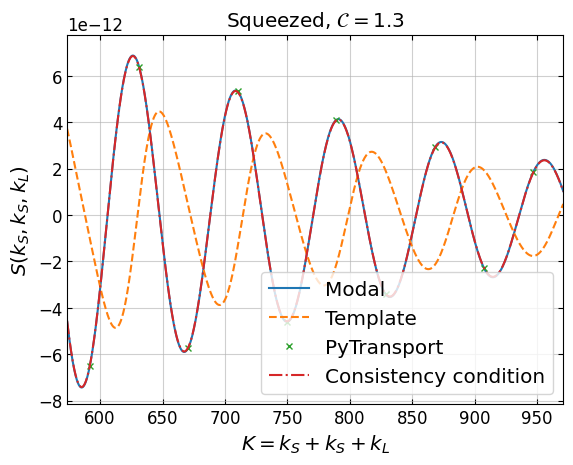
\includegraphics[width=0.49\columnwidth]{plots/tanh_5e-03_sqz}}
\caption{
	In the equilateral limit for the feature models (the top two figures) we validate our modal result
	against the PyTransport result. In the squeezed limit (the bottom two figures)
	we validate against PyTransport, and the consistency condition.
	In both limits, for both step sizes shown, we find excellent agreement.
	For the small step size (the two plots to the left), we additionally
	see a good match to the template of~\cite{adshead}. For the larger step size,
	the template amplitude is still accurate,
    but no longer captures the detailed shape information.
    This validates our code on non-Gaussianity generated by sharp
    features, and illustrates the general usefulness of our method.
	Our numerical results are accurate in a broader range than
	approximate templates, but are still smooth separable functions,
	unlike the results of previous numerical codes.
}\label{fig:tanh_sqz}
\end{figure*}
\begin{figure}[!pth]
\centering
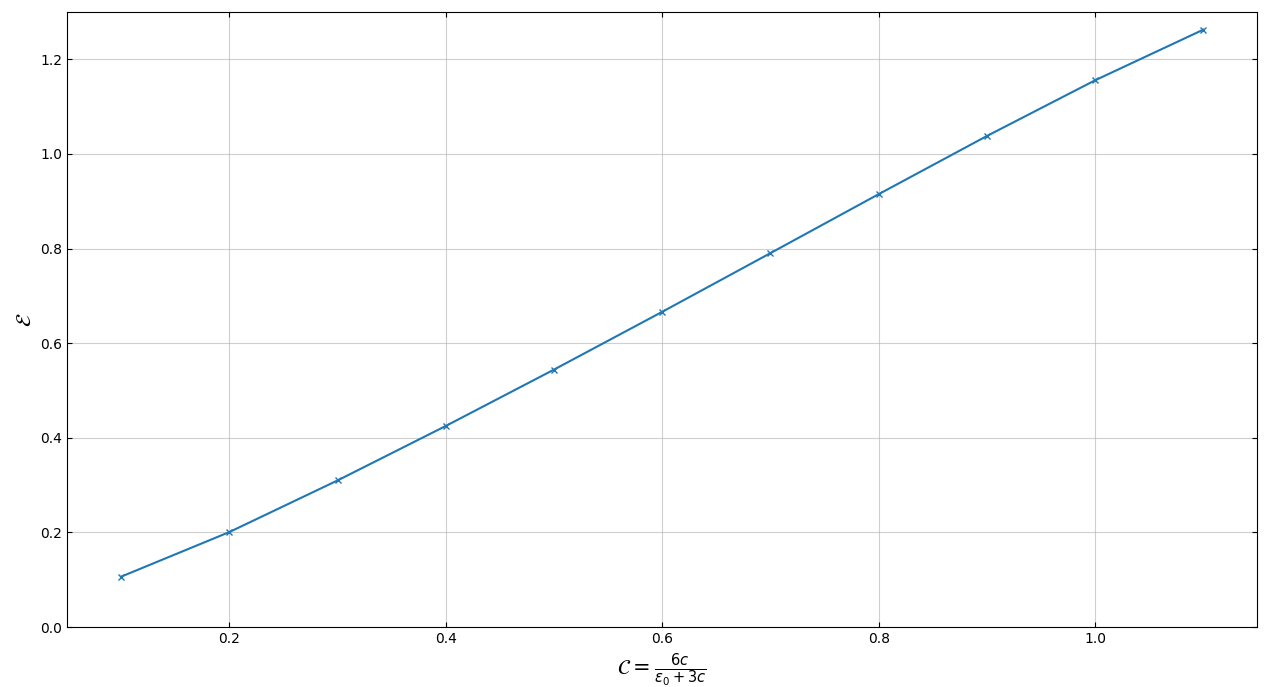
\includegraphics[width=.75\columnwidth]{plots/tanh_scan_C_cropped.png}
\caption{
    We sample more shapes with step sizes between the two
    feature models shown in figure~\ref{slice_plot_tanh}.
    We plot the relative difference,
    integrated over the full tetrapyd
    in the sense of~\eqref{relative_difference},
    between the modal result and the analytic template of~\cite{adshead},
    as a function of the template parameter $\mathcal{C}=\frac{6c}{\varepsilon_0+3c}$
    (where $c$ is the step size and $\varepsilon_0$ is the value of the slow-roll parameter
    $\varepsilon$ at $\phi_{step}$ when $c=0$). We test our result by verifying
    the squeezed limit consistency
    condition to better than 1\% throughout (not shown). The number of oscillations in the
    $k$-range is determined by the conformal time at which the kink in~\eqref{eq:kink_potential}
    occurs, which is kept constant across this scan. The width of the feature was also kept constant.
}\label{fig:tanh_scan}
\end{figure}

\subsection{Resonance features}
Now we further validate our code against two
resonance models. In contrast to the previous sharp kink,
this feature is extended, requiring precision at earlier times.
The first, shown in figure~\ref{pytr_comparison_min},
is a model with a canonical kinetic term, on a
quadratic potential with a superimposed
oscillation~\eqref{eq:resonant_potential}.
We take $bf=10^{-7}$, and $f=10^{-2}$.
The resulting bispectrum has oscillations logarithmic in $k_1+k_2+k_3$.
In figure~\ref{pytr_comparison_min} we see the excellent agreement
between our result and the PyTransport result, once initial conditions
in both codes are set early enough to achieve convergence.
This validates the code on non-Gaussianity generated deeper
in the horizon. Note the change of phase in the squeezed limit,
though this is expected to be unobservable.
We obtain a full tetrapyd convergence test result
(between $\Pmax=65$ and $\Pmax=35$)
of $0.93\%$, a squeezed limit test result of $1.1\%$
(along the line defined by~\eqref{sqz_line}),
and a relative difference of $3.0\%$ with respect to the
PyTransport result,
although this is only integrated over the two-dimensional slice presented in
figure~\ref{pytr_comparison_min}.


The time taken for the PyTransport code (per configuration) varies by a factor of around forty
between the equilateral limit and the squeezed limit,
as we show in figure~\ref{pytr_comparison_min}.
While the PyTransport code is extremely fast at calculating the shape function
for a single $k$-configuration,
to obtain this two-dimensional slice through the tetrapyd took around seven hours;
to obtain the shape function on the full three-dimensional tetrapyd would take much longer.
In contrast, our code took less than an hour on the same machine to calculate
the full shape function, not limited to the shown slice.
The overall speed increase is, therefore, a factor on the order of $10^2$ to $10^3$
for the full shape information, speaking only on the level of primordial
phenomenology, in addition to the advantage that our result is in a form
designed to be compared with observation.
We expect that our implementation can be optimised beyond this.


The second scenario we consider here also has an
oscillation superimposed on its potential, but this time
is a non-canonical model, the DBI model.
The resulting bispectrum is shown in figure~\ref{slice_plot_dbi_reso}.
Note especially the out-of-phase oscillations in the flattened limit,
which are potentially observable.
For the purpose of displaying this phenomenology, we place a window
on the oscillation in the potential, smoothing out the resulting oscillations
in the shape at low $k_1+k_2+k_3$, to aid convergence.
This validates our code on non-Gaussianity generated by deviations from Bunch-Davies
behaviour~\cite{chen_folded_resonant,features_bartolo}.
We obtain a convergence test result (between $\Pmax=65$ and $\Pmax=35$)
of $0.15\%$, and a squeezed limit test result of $6.5\%$.


\begin{figure}[!pth]
\centering
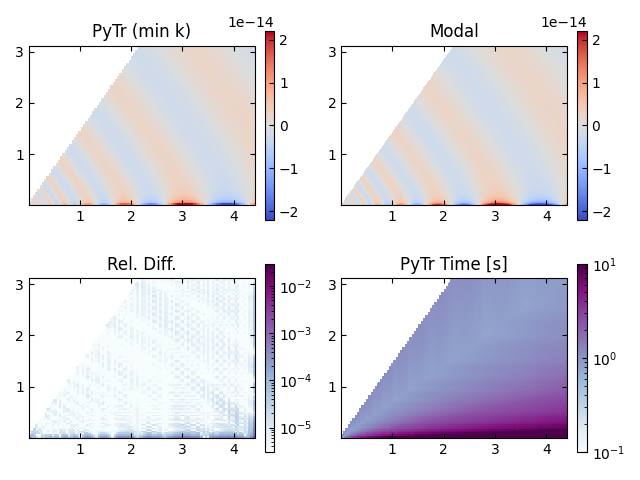
\includegraphics[width=0.99\columnwidth]{plots/slice_min_100.png}
\caption{
    Resonance on a quadratic potential~\eqref{eq:resonant_potential},
    testing our result using point tests against the
    PyTransport code.
    The logarithmic oscillations in the shape function are generated by periodic
    features deep in the horizon.
    The differences between our result and the PyTransport result
    are sufficiently small throughout that we can consider this
    a validation of our code on non-Gaussianity generated by periodic
    features deep in the horizon.
    In the $\Lnsboth$ basis, with $n_s^{*}-1 = -0.0325$,
    our result has a relative difference of $9.6\times10^{-3}$
    % 9.5587e-03
    between $\Pmax=65$ and $\Pmax=35$.
}\label{pytr_comparison_min}
\end{figure}

\begin{figure}[!pth]
\centering
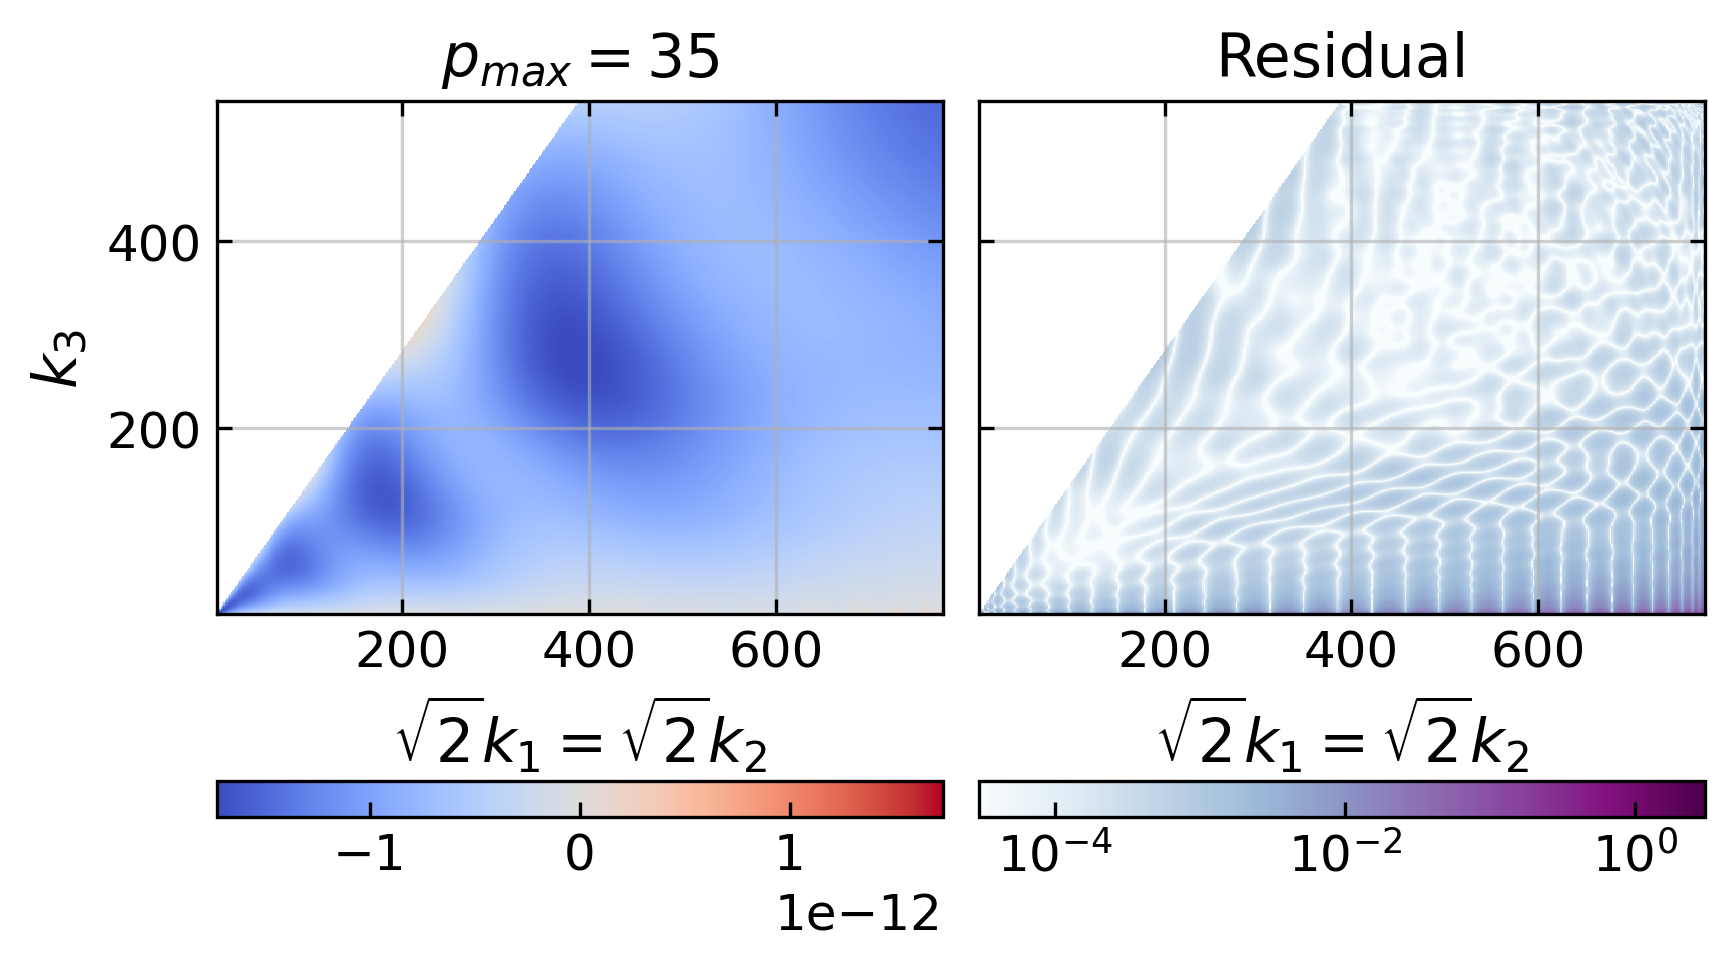
\includegraphics[width=0.99\columnwidth]{plots/tetra_slice_dbi_reso_bump_hq_coolwarm.png}
\caption{
    Non-Gaussianity generated by periodic
    features in a DBI model, including a phase difference
    in the flattened limit as described in~\cite{chen_folded_resonant}.
    For the purposes of demonstrating the phenomenology,
    we have placed an envelope on the oscillations in the potential
    to aid convergence.
    In the $\Lnsboth$ basis, with $n_s^{*}-1 = -0.0325$,
    the result has a relative difference of $1.9\times10^{-3}$
    % 1.9482e-03
    between $\Pmax=65$ and $\Pmax=35$.
}\label{slice_plot_dbi_reso}
\end{figure}

\section{Speed comparison vs PyTransport. Something BINGO can't do?}
\section{Map distinguishability of templates at primordial level}
    \subsection{Determine where to usefully scan.}
\section{Conclusion}
    \subsection{My methods (and their implementation) have been validated on interesting examples.}
    \subsection{Have successfully developed separable methods for high orders and features for the first time.}
    \subsection{Can obtain full shape info far faster than previous numerical methods.}

%\bibliographystyle{unsrt}
%\bibliographystyle{JHEP}
%\bibliography{thesis}
